
\documentclass{article}
\usepackage{CJK}
\usepackage{multicol}
\usepackage[margin=1in]{geometry}% Change the margins here if you wish.
\setlength{\parskip}{5pt} % This sets the distance between paragraphs
\usepackage[utf8]{inputenc}
\usepackage{amsmath}
\usepackage{mathtools}
\usepackage[framed,numbered,autolinebreaks]{mcode}
\usepackage{physics}
\usepackage{graphicx}
\usepackage{siunitx}
\usepackage{caption}
 \usepackage{hyperref}
\usepackage{listings}

\newenvironment{figurehere} 
    {\def\@captype{figure}} 
    {} 
\makeatother%用于连接公式编号

\usepackage{enumitem}
\setenumerate[1]{itemsep=0pt,partopsep=0pt,parsep=\parskip,topsep=5pt}
\setitemize[1]{itemsep=0pt,partopsep=0pt,parsep=\parskip,topsep=5pt}
\setdescription{itemsep=0pt,partopsep=0pt,parsep=\parskip,topsep=5pt}


\title{EECS C206B: Project 4

Grasp Planning with Sawyer

}
\author{Submitter: Enyang Zou, Tianqi Zeng, Encheng Liu}
\date{\today}

\begin{document}
\large
\maketitle

\section{Abstract}
In this project, we developed and implemented three grasping planning algorithms: Gravity Resistance, Ferrari-Canny, and Robust Force Closure, in both simulation and on the Sawyer. We started by implementing the discretized friction cone and calculated the grasp quality for each case. For the results, we got 5 graphs for each object, and they indicated the different applicable grasping points for each object. 

We finished our code in the given grasping.py, setting different threshold into the function we set, and using cvxpy to solve the convex optimization problem. It demonstrated that the effectiveness for our grasping algorithm. 



\begin{multicols}{2} 
\section{Methods}
In this section, we will explain in detail our approach towards each of the three grasp planning algorithms, and address the necessary concerns on it. 
\subsection{Extra Credit}
In the simulation, we can directly get the pose and position of the cube by calling the vertices or the mesh parameters. And all the grasper pose is also regarding to the absolute coordinate--the central point of the given objects. 

But in the real world, things are different. The pose we input to the robot is based on the robot base\_link, which is different from the object itself. And there is no TF tree transformers for us to do such a transformation.

We found two way to solve the problem, recalibrating the object position regarding to the robot base\_link. 
\begin{itemize}
    \item Using AR\_tag and AR\_tag TF Transformer just as Project1, visual Server

We put an AR\_tag near the object, look up and record the AR\_tag's position regarding the robot base\_link, and then manually estimated and calculate the optimal position of the object

    \item  Manually pulling the robot Tool Center to put on the object surface, and then use TF tree echo to show the right\_hand\_gripper position. This method is also really time-consuming. But it can works for serveral times
    
\end{itemize}




\subsection{Grasp Metrics}


\subsubsection{Gravity Resistance:} 

In order to calculate the gravity resistance of a grasp, we are supposed to solve the optimization problem in order to minimize the perpendicular finger force applied by the fingers while countering the gravitational force acting on the object, which is implemented by the function contact\_forces\_exist().


By the hints given in google doc, we figured it out that the target forces fc consists two set of individual force, one for grasp1 and one for grasp2. So that we can separately set the constraints on it. 

\begin{minipage}{\linewidth}
\centering
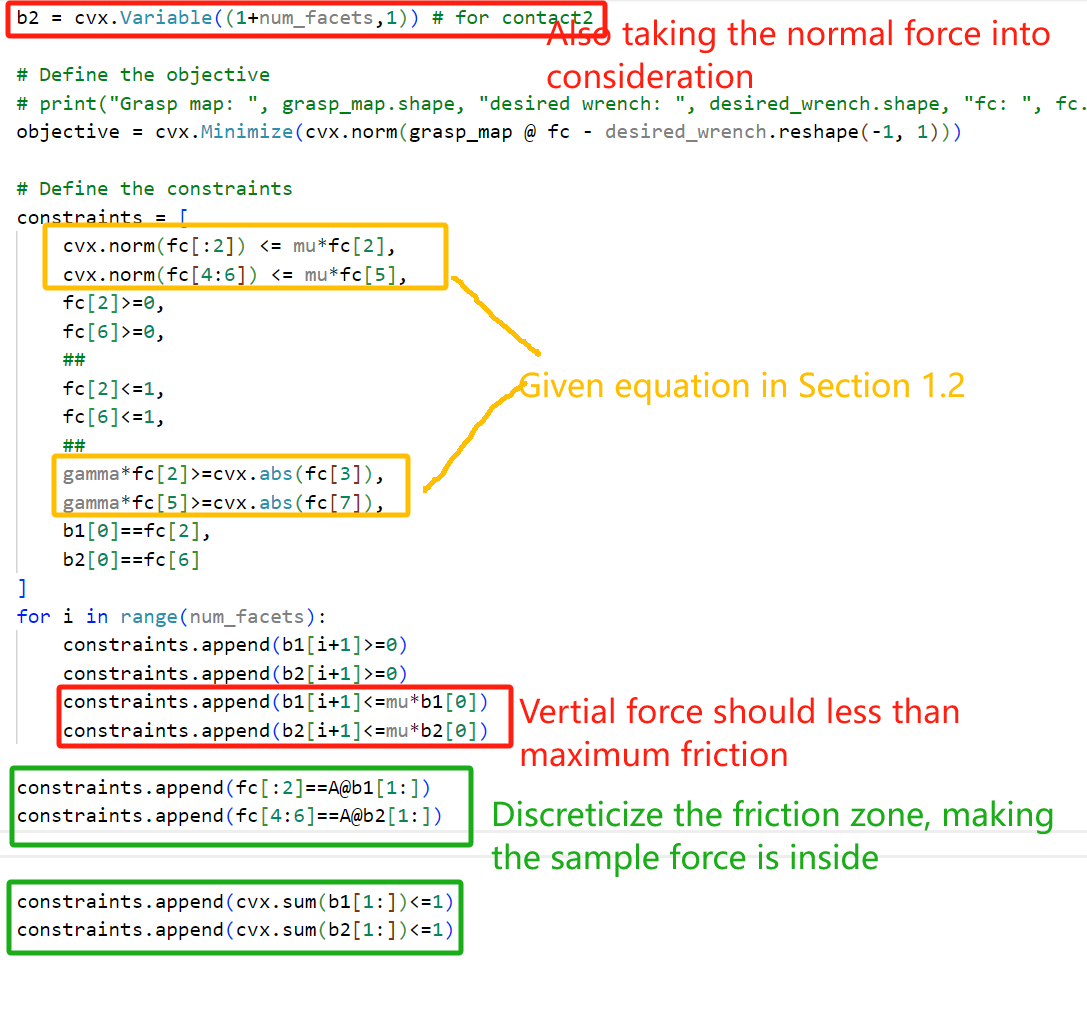
\includegraphics[width=7.8cm]{contactForceExist.png}
\captionof{figure}{Constraint Configuration}
\label{contactForceExist Constraint Configuration}
\end{minipage}

To do so, We discretized the friction cone into a pyramid with n vertice to convert so that we converted the non-convex problem into a convex one to do the optimization. This was achieved by representing the friction cone as a set of linear constraints using a composite matrix with the edges of the pyramid as its columns. 

The dimension for A is 2*num\_facets, the dimension of fc is 8*1, the dimension for b1 and b2 is (num\_facets+1) here.



\subsubsection{Ferrari-Canny}

The Ferrari-Canny metric is method that measures how much force that is required for a grasp to maintain force closure. In the implementation, we use cvxpy Python package to solve the optimization problem. The quality of the grasp is determined based on the minimum radius calculation, reflecting the stability and force-closure properties of the grasp.\cite{RUBERT2019103274}

Here is how we solve the problem.


\begin{itemize}
    \item Gravity Wrench Calculation
    \item Iterative Trial Approach
    \item Checking Contact Forces
    \item Minimum Sphere Radius\cite{219918}
    \item Quality Assessment
    \item Return Score
    
\end{itemize}

To begin, the gravity wrench was calculated based on the object's mass and the gravitational acceleration. Subsequently, an iterative trial approach was employed, conducting multiple trials to add random noise to the wrench and verify the existence of contact forces\cite{Graspqualitymeasures:}. In our implementation, we take 10 trials to get it. And then we use contact\_forces\_exist() to check if the force exist.

In assessing the quality of the grasp, if the minimum radius remained infinite after all trials, it indicated a lack of force-closure, leading to a quality score of zero. Conversely, the quality of the grasp was inversely proportional to the minimum radius, reflecting greater stability with a smaller radius.

\subsubsection{Robust Force Closure} 

The implementation of the grasp metric involves assessing the robust force closure by evaluating the quality of a grasp based on the given parameters.

 The function takes input parameters including mesh vertices, normals, the number of facets for friction cone approximation, coefficient of friction m, torsional friction coefficient gamma, and the mass of the object\cite{Graspqualitymeasures:}.

In this implementation, the optimized backend for solving the convex optimization problem is not explicitly specified in the provided code snippet; however, we utilized the cvxpy Python package for convex optimization\cite{8202167}.


Additionally, within the function, random disturbances were added to the pose of the object for multiple samples (specified by num\_samples) to evaluate the force closure for each disturbed pose. The quality of the grasp was then determined based on the proportion of successful grasps over the total number of samples.

The selected parameters, num\_samples=500, mu, gamma, and object\_mass were chosen to ensure a robust evaluation of the grasp quality. The number of samples influences the robustness of the evaluation, while the coefficients of friction and the object's mass impact the stability and quality of the grasp.




\subsection{Description of grasp planning algorithm}

In our grasp planning algorithm, we aim to determine a robotic gripper's pose that will enable a secure grasp of an object, given the mesh representation of the object and a predefined set of contact points. Our method involves conducting a series of trials to identify a grasp that meets force closure criteria and quality metrics.

Throughout each trial, the following steps are undertaken:

\begin{enumerate}
\item Perturb the initial contact points along their respective surface normals to generate a variety of potential grasps.
\item Evaluate the perturbed contact points for force closure to ensure the grasp can withstand external forces.
\item Measure the potential grasp against three critical metrics: gravity resistance, the Ferrari-Canny metric for grasp quality, and robust force closure.
\end{enumerate}

Should the contact points satisfy our evaluation thresholds, we compute the gripper's pose. This pose is encapsulated in a 4x4 transformation matrix that combines both the necessary position and orientation for the gripper to perform the grasp:

\begin{equation}
\text{Gripper Pose} = \begin{bmatrix}
R_{11} & R_{12} & R_{13} & p_x \\
R_{21} & R_{22} & R_{23} & p_y \\
R_{31} & R_{32} & R_{33} & p_z \\
0 & 0 & 0 & 1
\end{bmatrix}
\end{equation}

Here, 
$\mathbf{R}$ denotes the rotation matrix derived from the normals at the contact points, and $\mathbf{P}$
  is the centroid of the perturbed contact points, dictating the gripper's position. If our algorithm does not find a suitable grasp after a set number of trials, we return \texttt{None}. This result suggests that under the current constraints, a feasible grasp is not attainable, prompting a reevaluation of the contact points or the object's graspability.





\section{Experimental Results}
In this part, we will provide a set of figures for each object

\subsection{Extra Credit}


\subsection{Graphs and Videos}
These are the records the scores of each of your planned grasps for each of the three different grasp
metrics


\href{https://drive.google.com/file/d/1GXad7t8-8eQQp-zyBbwTg42D6n97q5GY/view?usp=drive_link}{ Here is Lab Video, including Grasp on Nozzle and Pawn}
\begin{center}
\begin{tabular}{ | m{1.5cm} | m{1.5cm}| m{1.5cm}| m{1.5cm}|  } 
\hline
&Gravity Resistance & Ferrari-Canny & Robust Force\\
\hline
Pawn & 1.0 &  0.4123 & 0.7123\\
\hline
 & 1.0 &  0.4431 & 0.7754\\
\hline
 & 1.0 &  0.4442 & 0.7865\\
\hline
 & 1.0 &  0.4478 & 0.7375\\
\hline
 & 1.0 &  0.4486 & 0.7875\\
\hline
 & 1.0 &  0.4480 & 0.7343\\
\hline
 & 1.0 &  0.4548 & 0.7765\\
\hline
 & 1.0 &  0.4575& 0.7264\\
\hline
 & 1.0 &  0.4389& 0.7865\\
\hline
 & 1.0 &  0.4547 & 0.75768\\
\hline
  & 1.0 &  0.4547 & 0.7382\\
\hline
  & 1.0 &  0.4489 & 0.876\\
\hline
  & 1.0 &  0.4482 & 0.7259\\
\hline
  & 1.0 &  0.4485 & 0.7378\\
\hline
   & 1.0 &  0.4326 & 0.7861\\
\hline
  & 1.0 &  0.4496 & 0.73836\\
\hline
  & 1.0 &  0.4445 & 0.73836\\
\hline
Nozzle & 1.0 & 0.4523 & 0.6153 \\
 \hline
  & 1.0 & 0.4523 & 0.62634 \\
 \hline
  & 1.0 & 0.4567 & 0.6462 \\
 \hline
  & 1.0 & 0.4568& 0.67885 \\
 \hline
  & 1.0 & 0.4583 & 0.64587 \\
 \hline
  & 1.0 & 0.4527 & 0.68347 \\
 \hline
  & 1.0 & 0.4485 & 0.63475 \\
 \hline
  & 1.0 & 0.4375 & 0.68246\\
 \hline
  & 1.0 & 0.4557 & 0.68477 \\
 \hline
  & 1.0 & 0.4476 & 0.68347 \\
 \hline
  & 1.0 & 0.4568 & 0.68864 \\
 \hline
  & 1.0 & 0.4597 & 0.68089 \\
 \hline
  & 1.0 & 0.4537 & 0.68374 \\
 \hline
  & 1.0 & 0.4527 & 0.6783 \\
 \hline
  & 1.0 & 0.4596 & 0.67990 \\
 \hline

\end{tabular}  
\end{center}


\subsection{Object Scores and results}
In general, the results for gravity resistance have a perfect score, 1, which is much better than Ferrari-Canny, which is around 0.4. This might be wrong for gravity resistance because it seems impossible to get everything correct in the two force metrics. 



\section{Discussion}
\subsection{Problem 1}
\textbf{Discuss how performance differed across the objects. Which object was the hardest? Which was the easiest? Why?}

The pawn is the easiest to grasp, and the nozzle is the hardest one. I think this my result from several aspects.

\begin{itemize}
    \item The overall size of nozzle is smaller that pawn, making it harder for robot to locate
    \item The surface of pawn is more flat than nozzle, making the friction zone and feasible torque more restricted in nozzle than pawn
    \item For the localization, pawn is taller than the nozzle, which provides a larger buffer space for pawn when robot is moving or grasping.
\end{itemize}




\subsection{Problem 2}
\textbf{ Discuss what difficulties you faced when designing your grasp planning algorithm. Were there any edge cases you did not anticipate?}


Yes, We face a lot of problems when implementing the grasp planning algorithm. 

\subsubsection{Difficulties when setting constraint on force exist functions}
The first problem we met is to setting the dimension of Variable fc in the function contact\_force\_exist. Because the grasp\_map is a 6*8 matrix, so fc should be a 8*n matrix to make the result feasible. And from the lab doc, we know that fc consist of four individual components, from f1 to f4. So at the very beginning, we just set fc to be a 8*4 matrix, which caused a strong confusion. After rethinking our code, we found that we can divide the fc into two parts, the first 4 elements for the first grasp, the last 4 elements for the second grasp.

But after we figured out how to solve the problem, we found the solution to the convex optimization problem is always feasible. Which means the score returned by robust closure is always 1. Really strange on it. To fix this issue, we found that when we designing our constraint, we forgot to add the sum of alpha\_i is less than 1. After adding several corner cases, our result could be normal now. 

\subsubsection{Difficulties when Implementing the grasp into real world}

As mentioned before, the function custom\_grasp\_planner just returned the pose regarding the object frame. But for a real world robot, it should return a pose regarding the robot base\_link frame. It's really hard to find the object position in a real world. 

To integrate the simulation code into the real-world control. We move all the databag from the simulation, such as the surfaces meshes, the grasp vertices and etc. We use 206A Lab 5's code and try to modify it to call the custom\_grasp\_planner to get the grasp pose. 

\begin{lstlisting}[language=Python]
#how to change the pose from object's reference frame to the robot r
'''
- Translation: [0.744, 0.175, -0.132]
- Rotation: in Quaternion [0.034, 0.996, -0.031, 0.080]
            in RPY (radian) [-3.084, 0.163, 3.078]
            in RPY (degree) [-176.674, 9.320, 176.383]
'''
object_pose_translation = np.array([0.744, 0.175, -0.132])
object_pose_rotation = tf_trans.quaternion_matrix([0.034, 0.996, -0.031, 0.080])

# Combine the translation and rotation into a single 4x4 transformation matrix
object_pose_in_base_link = np.dot(tf_trans.translation_matrix
(object_pose_translation), object_pose_rotation)
\end{lstlisting}

We also use AR\_tag to implement it. 


\subsection{Problem 3}
\textbf{Discuss the strengths and limitations of your custom grasp planning algorithm. Do you use any heuristics
that depend on assumptions that may not always hold? Is your planner computationally efficient? Can you think of any failure cases for your planner?}

The custom grasp planning algorithm has several strengths. It uses a series of trials to identify a grasp that meets force closure criteria and quality metrics, which allows it to generate a variety of potential grasps. It also uses a transformation matrix to compute the gripper's pose, which combines both the necessary position and orientation for the gripper to perform the grasp. However, the algorithm has some limitations. It assumes that the contact points satisfy the evaluation thresholds, which may not always be the case. Additionally, the algorithm may not be computationally efficient if a suitable grasp is not found after a set number of trials. A potential failure case for the planner could be when the object's graspability is low, prompting a re-evaluation of the contact points or the object's graspability.

\subsection{Problem 4}
\subsubsection{Discuss any physical principles that appear to differentiate the successful grasps from the failures.}


As for physical principles that appear to differentiate the successful grasps from the failures. According to our observations in the lab, for the nozzle object, when the grasp planner are giving grasps on the two sides with acute inclination angle, the grasp are failing. This is because the grasp force on the vertical direction cannot cancel the gravity. However, the calculation metric may give a feasible result because we are meshing finite points on the surface thus only calculating the approximating normal and vertices. The real grasp cannot land on the exact planned the point. 

And when they grasp such acute inclining area, the grasp will fail due to the physical principal. Also, as we are having a soft contact gripper, we can see that when we are trying the grip the ball on the pawn from two side directions, it always goes smoothly, as the part of the sphere surface is similar; so the minor error in the gripper position do not influence the physical law as the part of the soft fingers are contacting the lower semisphere and resulting in a upward composite vertical force cancelling the gravity.    

\subsubsection{Discuss how predictive each of your grasp metrics were for the success or failure rate of the given grasps}

 The grasp metrics were somewhat predictive for the success or failure rate of the given grasps. The gravity resistance metric consistently scored perfect, which may indicate that it is not a reliable predictor of grasp success. The Ferrari-Canny metric and the robust force closure metric had more varied scores, which may make them more reliable predictors of grasp success. However, these metrics are based on mathematical models and may not fully capture the complexities of real-world grasping.


\subsubsection{Do the grasp metrics seem to have predictive power? Or do the grasps seem to succeed/fail in real life for other reasons}

The grasp metrics do seem to have some predictive power, as they provide a quantitative measure of the grasp's quality. However, the success or failure of grasps in real life can also be influenced by other factors not captured by these metrics. For example, the physical properties of the object and the gripper, such as their size, shape, and material, can significantly affect the success of a grasp. Additionally, the accuracy of the robot's movements and the stability of its grip can also impact the outcome of a grasp.

\subsection{Problem 5}
\textbf{Discuss what worked well for the grasping pipeline, and what could be improved.}


Our grasp planning algorithm contains several parts: generate potential grasp, evaluate potential grasps with three metrics and return the gripper pose for the grasp to execute. There are several points to be further optimized. The first one is the restrictions implemented the force closure method, we are implementing some restrictions that may be able to express in matrix form with the form of a for loop, which is increasing the restriction number and potentially add burden to the computer. The second  point is that we may be able to justify and maybe delete some of our restrictions to relief the calculation burden.

For the whole program, it make take 5 minutes to run, forcing our group member to stay in the lab for a long time. The third point about this is that we may use other more efficient packages to enhance the optimization efficiency itself. Another concern is about the inverse kinematics. If we change the end pose too much, great chances are that the program giving unsolvable as the result. The inverse kinematic method we are using is naive to some extent, we should try either using multi-steps of motions or more complicated algorithm with bigger feasible space. 











\pagebreak
\appendix
\section{Bibliography}
\bibliographystyle{plain}
\bibliography{Reference}
\section{Appendix}
\subsection{Useful Links}
\href{https://github.com/ucb-ee106-classrooms/projects-3-4-ambulance/tree/master/project4}{GithubLinks}


\subsection{Reflection on this project(Bonus)}
The first point is that the conversion from the mathematical model to the real coding, especially the friction cone part. At first, the variable names vertices, f, fc are all very similar and confuse us a lot. Confusion between vertices as contact points of the gripper and the object and the decomposition of friction cone into a 3D polynomial which has a lot of vertices give rise to a lot of bugs. Similar questions require us to be more familiar to the basic algorithms and principals. Actually, we managed to code again correctly after reading through this chapter is MLS together.

The second point is about the manipulation of quaternion in python. We initially want to install the quaternion package on the lab computer, but we found we do not have the access to download packages. So we have to write more codes to do the calculation in a more conplex way. We understand this restriction is makde out of safety concerns. So, maybe it would be a good idea to prepare this package in the computer next semester.

The last point is about the mental one. As we have mentioned, we was confused and frustrated at first. And we are nearly giving up this lab. But when we encourage ourselves to learn again from the MLS chapter, we came back and basically completed this lab. Some problems may seem to be impossible to solve at one time, but if we keep trying, they will be solvable.

\end{multicols}
\end{document}
